\subsection{ERROR REDUCTION}

In this section, we discuss error in analysis of images. The target has differents forms. However, 
ROI is rectangular window. Certains areas more importants were identified inside of ROI.
In Fig. \ref{fig:erroridentified}, there are any areas close of edges that target not occupies. They are
considered like error areas.

\begin{figure}[H]
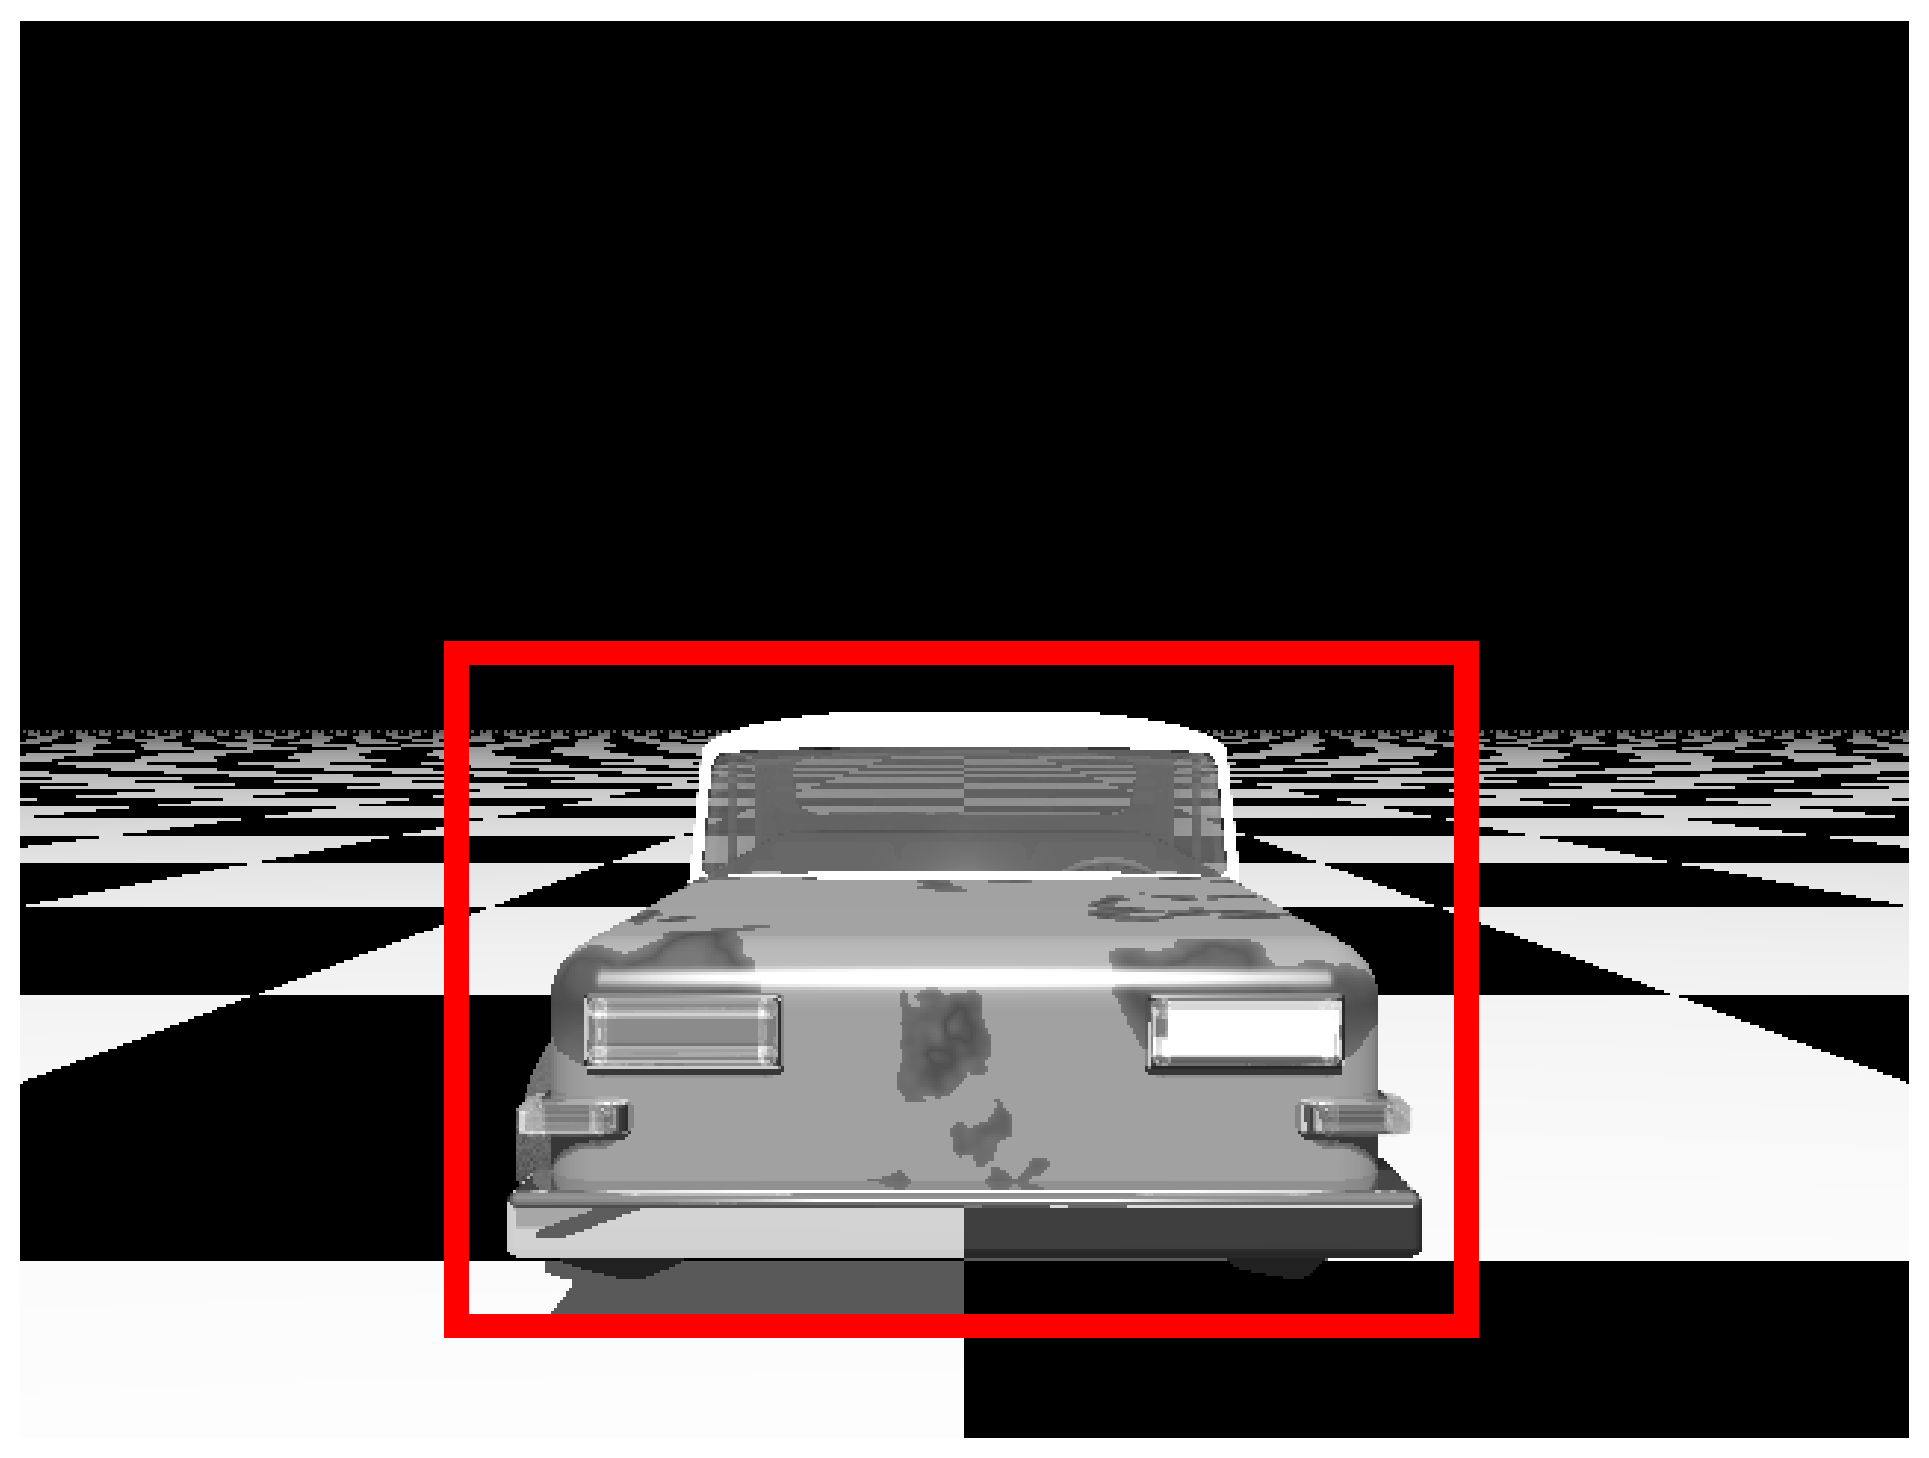
\includegraphics[width=\columnwidth]{images/imageError.eps}
\caption{Illustration of ROI with error areas close of edge.}
\label{fig:erroridentified}
\end{figure}

Two matrix at same dimensios can be compared in PCC. This method of comparesion doesn't generate
any date if dimensions of frame are equals. 
We are also interested to use in several applications PCC because this method has high precision.

We decide solve this problem given a ponderation in PCC. Then, points on the target was considered plus important
and points out of target has less importance in correlation.

\begin{figure}[H]
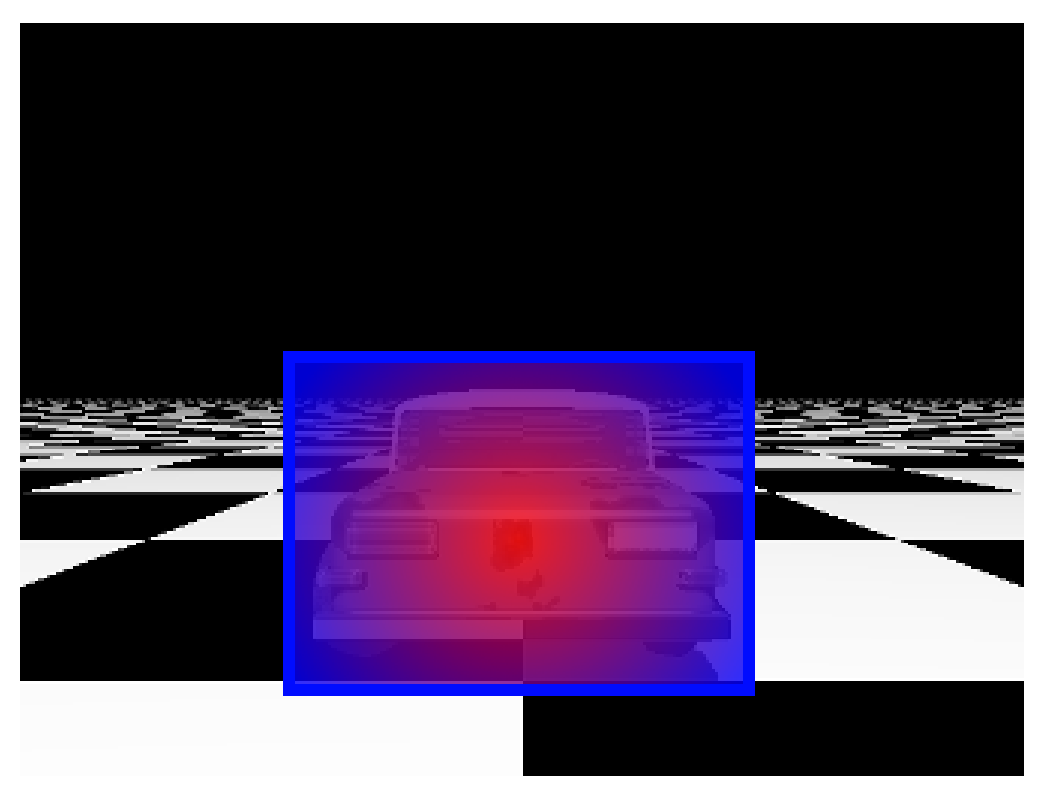
\includegraphics[width=\columnwidth]{images/imageErrorcontroled.eps}
\caption{Illustration of points of most importance (red) and points less importance (blue) in correlation.}
\label{fig:errorpondered}
\end{figure}

Points close of edge have less importance and they are in blue in Fig. \ref{fig:errorpondered}. 
Points close of center of image are red and, probably, they is on the object. This figure helps 
to illustrate the application of pondered PCC.